\chapter{Case Study -- Analysis of Power Consumption Dataset}

In recent years, we observe widespread IoT technologies in everyday life due to the decreasing price of smart sensors and high-quality network availability. Electricity distribution and consumption are no exception, and smart electric meters are now standard components in modern households. It eventually leads to a large amount of sensor data structured as time series, and there is a need for efficient analysis tools to process this information. 

As a part of our research in Gauss Algorithmic \footnote{\url{https://www.gaussalgo.com/}}, we got an opportunity to analyze such a dataset. Our assignment was to analyze, find clusters, and detect anomalies in a large dataset of power consumption curves, emphasizing their long-term behavior. We decided to prepare an end-to-end analytic pipeline for this dataset, from the initial data processing to the final outcomes,  that can be further used by other data scientists in their studies.

This chapter will go through all steps in our analytic pipeline on the power consumption dataset using techniques mentioned in the previous chapters and will propose a novel approach for time series transformation.

\section{Dataset Description}
First we will describe in detail the dataset that was used within this thesis. Our dataset consists of a large set of power consumption curves for customers located in Slovakia. Because of the strong emphasis on customers' privacy, all data are completely anonymous. We have only randomly generated numbers from our contracting authority representing customer labels and power consumption curves for every consumer. Thus, we lack information about the customer's location or type (apartment, household, company). We have over 20~000 time series from the February 1st 2017 to August 1st 2018. The sampling rate of our time series is one value in 15 minutes.

This initial step in our analysis aims to determine the quality of input data in terms of missing values, extremes, and dataset size. We found a high rate of incorrect or missing data. There are entirely missing days throughout the period and even several months in 2018 (Fig.~\ref{fig:dataset-example}). On average, we have approximately 52~000 data points, which corresponds to almost 547 days for each customer. In the end, we removed a portion of power consumption curves because they had only a few to none uncorrupted values, leaving us with over 12~000 time series for further analysis.
\begin{figure}[h]
    \centering
    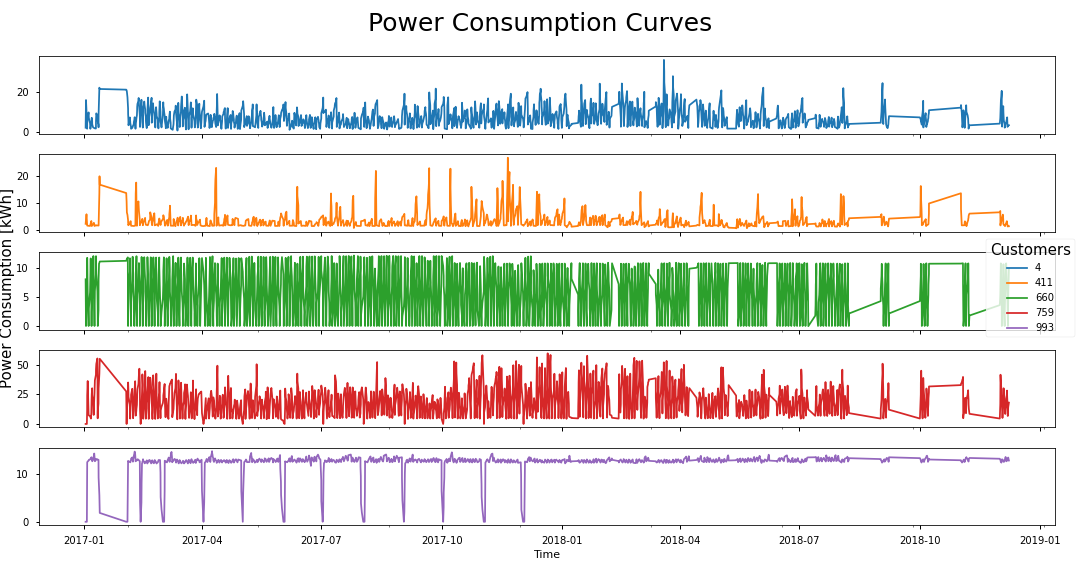
\includegraphics[width=\textwidth]{img/dataset-example.png}
    \caption{Example of power consumption curves with missing values and significantly different behavior.}
    \label{fig:dataset-example}
\end{figure}


\section{Requirements}

With our dataset's detailed overlook, we will divide our work into two objectives to accomplish our assignment. The first objective is to process the dataset into a form that could be easily analyzed (\textit{Data Engineering}), and the second goal is to perform the analysis -- clustering and anomaly detection with an emphasis on their long-term behavior (\textit{Data Analysis}).

\begin{enumerate}
    \item \textbf{Data Engineering:} A combination of rapidly changing customer power consumption, sensor errors, changes based on external factors, such as time of the year, and lack of information about a customer makes this task remarkably challenging. Another critical detail is the size of our dataset and the length of individual time series. To explore and analyze this data, we have to prepare the following steps: propose preprocessing and feature extraction resistant to missing data, extract long-term behavior, and maintain reasonable time and space complexity for all steps.
    \item \textbf{Data Analysis:} After the data preparation, we want to analyze our dataset and find outliers. As we are working with a large dataset of time series, we want to prepare meaningful views and visualizations, which will guide a user towards clusters and anomalous data.
\end{enumerate}

\section{Preprocessing}
We are working with a large number of data coming from smart electric meters. It is not unusual to encounter missing or unrealistic values due to sensor or network error. Therefore, it is essential to handle these types of defects in the preprocessing stage so they do not influence the results of the subsequent data analysis.

In our dataset, we distinguish between two unrealistic value cases: values with negative power consumption and sudden dramatic change in power consumption only for a single data point. It is not uncommon to observe a combination of both in one power consumption curve. We assume that this type of error is due to sensor or network failure. To deal with values below zero, we replace them with float \textit{nan} (not a number), representing the missing value. To remove value jumps, we compute our power curve's second derivation and replace values with a disproportionately large absolute value of the second derivation by \textit{nan} values.

We are not replacing the missing values with real numbers in our preprocessing step. Instead, we use the feature extraction technique that is resistant to them. We will address this problem in more detail in the next section.

\section{Feature Extraction}
Consumers' power consumption tends to change rapidly due to sudden extensive usage of electric devices, but it should be more stable in the long-term behavior. Thus we want to extract features that will reflect the long-term behavior and will not be significantly affected by swift changes. These features will provide a better overview of user behavior and make it possible to find users with similar power consumption. To overcome fluctuations of power in short periods, we want to study long-term periodic and non-periodic behavior. We do this by extracting seasonalities (periodic behavior) and trends (non-periodic behavior) in customer power consumption.

Due to the geological location and climate in Slovakia, power consumption is generally changing during the year. The main factors are changes in temperature and sunlight hours through seasons. To capture these changes, we extract weekly seasonality separately for every meteorological season. Another characteristic comes from daily seasonality, where we distinguish between free days and workdays. We also want to utilize trends and yearly seasonalities of our data. As holidays have a substantial impact on power consumption, we want to capture their effect in the model.

For extracting these seasonalities and trends from our data, we are using the Prophet by Facebook \cite{exp:FbProphet}. It uses a decomposable time series model with three main components: trend, seasonality, and holidays \cite{exp:lin-model}. It is formally defined as:
\begin{equation}
    y(t) = g(t) + s(t) + h(t) + \epsilon_t    
\end{equation}
Where $g(t)$ is the trend function, $s(t)$ is the seasonality function, $h(t)$ corresponds to the effects of holidays, and $\epsilon_t$ is noise keeping the normal distribution.

Prophet provides an interface to detect changepoints in trends automatically. However, because our data is relatively short, only eighteen months of data, we do not expect any significant trend changes in our data. Thus we are using a linear trend with zero change points. The Prophet uses the Fourier series representation to model multiple periodic effects (seasonalities) with different lengths. We use yearly seasonality, free day and workday daily seasonality, and weekly seasonality for every meteorological season. To include the effects of holidays, it uses a matrix of regressors corresponding to every holiday. This effect is also applied to days before and after the holiday. Other essential features are the ability to deal with missing values, computational speed, and scalability.

In this work, we manually define seasonalities based on the expected behavior of different customers based on the consultation with our contracting authority. First, we expect a different behavior on free days (holidays, weekends) and workdays. Then, because of the weather changes during the year, there can be a change in weekly behavior, so we are using a weekly seasonality for every season. Finally, we want to see the trend and the yearly seasonality. We can see the example of this decomposition in Fig.~\ref{fig:seasonalities}. Using this feature extraction allows us to find customers with similar properties in one seasonality but significantly different behavior in others -- for example, two customers with almost identical seasonalities but significantly higher power consumption could be a sign of energy theft.
\begin{figure}[h]
    \centering
    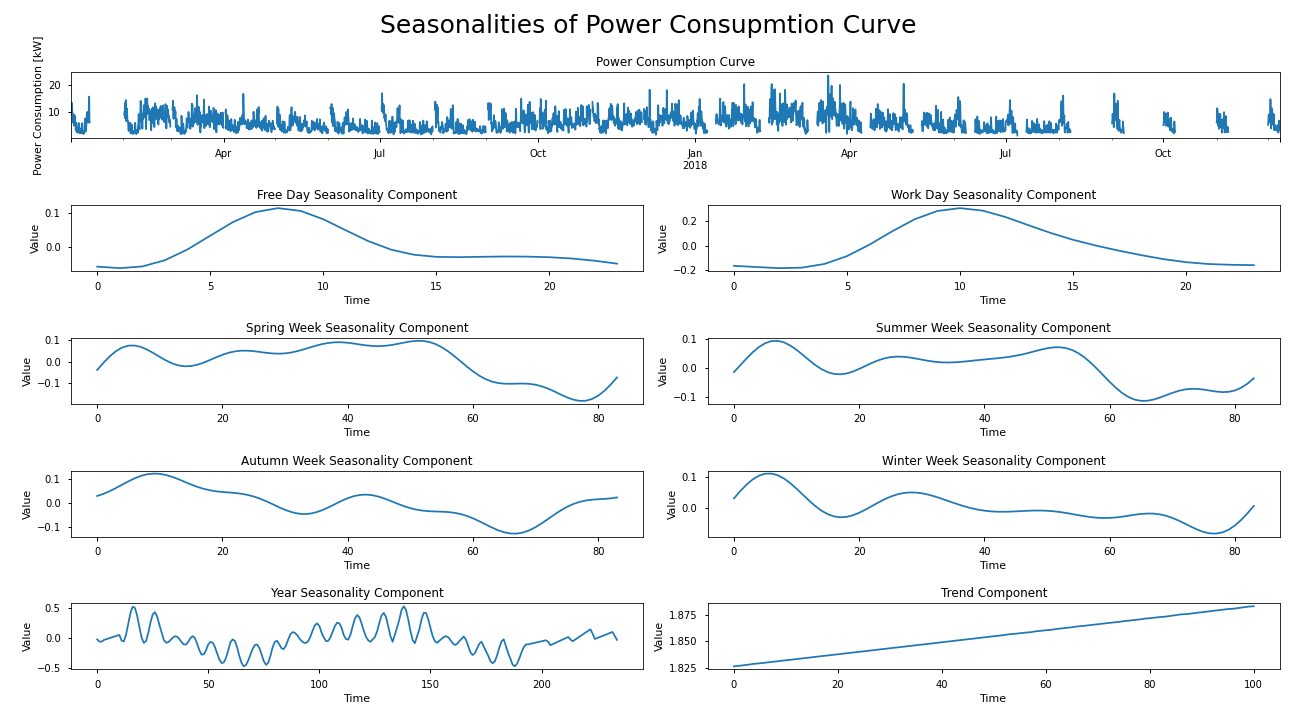
\includegraphics[width=\textwidth]{img/seasonalities.png}
    \caption{Example of seasonalities extracted from a single power consumption curve (top-most curve) from our dataset using the Prophet.}
    \label{fig:seasonalities}
\end{figure}

In summary, we are describing our original time series with eight new time series: free day and workday seasonalities, spring, summer, winter, and autumn weekly seasonalities, yearly seasonality, and trend. In the next section, we will provide techniques for combining information from time series with multiple components with different lengths (\textit{multi-component} or \textit{multi-model} time series) into a single representation.

\section{Interactive Feature Space Building}
Once we use seasonalities and trends, our dataset changes from univariate time series into a multi-component time series consisting of eight time series with different lengths and temporal resolution. Because of the lack of knowledge about the customer, we are working with unsupervised learning on a large dataset of multi-component time series. In our solution, we will first propose a technique for transforming this type of data into a spatial representation and then propose an optimized version of the technique for work with large datasets.

\subsection{Multi-Component Feature DTW Transformation}
We propose a novel technique called \textit{Multi-Component Feature DTW transformations (MCFDTW)} to transform the dataset of multi-component time series into a spatial representation. As Kate \cite{met:fDTW} has shown, it is possible to combine multiple Feature DTW transformations (FDTW). Similarly to his approach, the MCFDTW is a union of FDTW transformations for every component  of our multi-component time series.

Having a dataset $S = {T_0, T_1, \dots, T_n}$ of multi-component time series $T_n = (a_{n0}, a_{n1}, \dots, a_{nj})$, where $a_{nj}$ are time series of an arbitrary length and $A_j = (a_{0j}, a_{1j}, \dots, a_{nj})$ are tuples of time series from one component, we define the MCFDTW transformation as:
\begin{equation}
 MCFDTW(S) = ( FDTW(A_{0}) | FDTW(A_{1}) | \dots | FDTW(A_{j}) )
\end{equation}
where $|$ denotes a concatenation of feature matrices from FDTW transformations.

To increase the efficiency of MCFDTW, instead of the original FDTW transformation, we can use the Prototyped Feature DTW (PFDTW) as it is not computing whole distance matrices.

\subsection{Prototype Selection}
The prototypes are crucial for the success of PFDTW transformation, but their correct selection is a challenging task. Iwana et al. \cite{met:protofDTW} proposed two ways for the prototype selection from the full distance matrix for the dataset. The first one is using statistics to remove statistically insignificant feature vectors from the full distance matrix. This technique is usable in supervised and unsupervised learning, but it is impractical on large datasets because it requires the full distance matrix as a starting point. The second approach uses the AdaBoost algorithm to select the best features for classification, making it available only for supervised learning.

Because in our task, we are working with a large dataset and applying an unsupervised learning approach, we  are proposing several bottom-up methods for the prototype selection:
\begin{enumerate}
    \item Random selection
    \item Manual selection
    \item Selection by density
    \item Selection by Predicted Correlation
\end{enumerate}

\subsubsection{Random Selection}
The first and most straightforward option is to use randomly selected prototypes. This approach is very efficient, and if our sample is large enough, it covers a sufficient portion of the full feature space. Based on our tests on the UCR datasets \cite{exp:UCRArchive2018}, a random prototype selection seems to be a very efficient approach that still produces comparable results in terms of classification accuracy (Appendix~\ref{sec:app-ucr}). Because of these advantages, we recommend using this method of prototype selection as a starting point.

\subsubsection{Manual Selection}
The second approach is selecting specific time series as prototypes by hand. It is usable if the user has deep knowledge about the data and could pinpoint the significant time series. As the resulting feature vectors are the distances to these specific time series, it is easily interpretable for the user.

Even though using only manually selected prototypes has the advantage of additional explainability, the user could miss some important time series. To minimize this problem, we recommend combing manual selection with a random selection. If randomly selected prototypes improved the final results, we could suspect either that we selected improper prototypes or that our selection is too small.

In our pipeline, we are using the combination of dimensionality reduction methods and visualization for the manual selection of new prototypes (see \ref{sec:inter-fsb}~\nameref{sec:inter-fsb}).

\subsubsection{Selection by Density}
Another approach comes from an observation that we need more points to describe a dense region than the sparse one, similar to the Kohonen map \cite{exp:Kohonen1982}. This strategy starts with a random sample and then uses data visualization to select new prototypes from the dense regions and remove prototypes that are far away.

Because after the MCFDTW transformation, the transformed feature matrix has the number of dimensions equal to the number of selected prototypes, we can encounter the Curse of Dimensionality \cite{exp:curse-of-dim}. This is problematic for density-based techniques. Because there is no conventional solution to this issue, instead of using a fully automatic solution, we recommend to use a combination of dimensionality reduction and visualization techniques (see \ref{sec:inter-fsb}~\nameref{sec:inter-fsb}). Based on the work with our dataset, this approach yields stable results.

\subsubsection{Selection by Predicted Correlation}
As two strongly correlated feature vectors do not give much information from a statistical point of view, the last strategy we propose comes from an assumption that we could predict the correlation of potential new prototypes. To do so, we are using the correlations between currently selected prototypes and their feature vectors.

We start with the random prototype selection and transform the dataset into a feature matrix. Then we use Spearman's rank correlation coefficient and compute the correlation matrix between the feature vectors produced from our prototypes. Afterwards, we use the feature matrix and correlation coefficient of other prototypes to train a regressor to predict the correlation on other time series for each prototype. Finally, we select the prototypes with the lowest average predicted correlation.

Unfortunately, this method did not prove significantly better during our tests than the randomized selection of similar size. The prediction of the correlation of new prototypes was reasonably accurate, but it seems that the correlation was not the most reliable predictor of prototype quality. We think that there is an opportunity for future research direction.

\subsection{Interactive Feature Space Building}
\label{sec:inter-fsb}
Considering the techniques used for prototype selection, we split our feature space building process into an interactive iterative pipeline. The pipeline consists of six steps:
\begin{enumerate}
    \item Select a subsample of the dataset.
    \item Build a Prototyped Feature DTW space.
    \item Vizualize the dataset.
    \item Choose new or remove prototypes using the visualization.
    \item Repeat steps 2-4 until we are satisfied with the result or do not evidence any change.
    \item Apply MCFDTW to the whole dataset.
\end{enumerate}

Because our dataset consists of a large number of multi-component time series, we will randomly select a fraction of our dataset in the first step. We are using approximately one-third of our dataset, which allows us to work in real-time. As we expect large groups of similar power curves, the selection of this portion should consist of all major consumer groups, thus minimize the negative effect of not using the whole dataset.

In the second step, we are building the new feature space by using MDFDTW. In the first iteration, we are using the random selection of prototypes. After the first iteration, the feature space building is fully automatic based on the prototypes selected or removed in next step. As we are using the iterative approach, we do not recalculate already computed feature vectors, which increases the efficiency.

In the third step, we are selecting new prototypes using data visualizations. Firstly, we use PCA and UMAP/densMAP to visualize our dataset's global and local structures. As displayed in Fig.~\ref{fig:prototypes}, we can study the local and global structure of the dataset, including prototypes' positions. One point in Fig.~\ref{fig:prototypes} represents a single customer -- one multi-component time series. Using interactive zoom and selection, we can select time series to inspect them directly, study their position and surrounding in the UMAP and PCA transformations, and closely examine their seasonalities and trends (Fig.~\ref{fig:selected-seasonalities}). 
\begin{figure}[h]
    \centering
    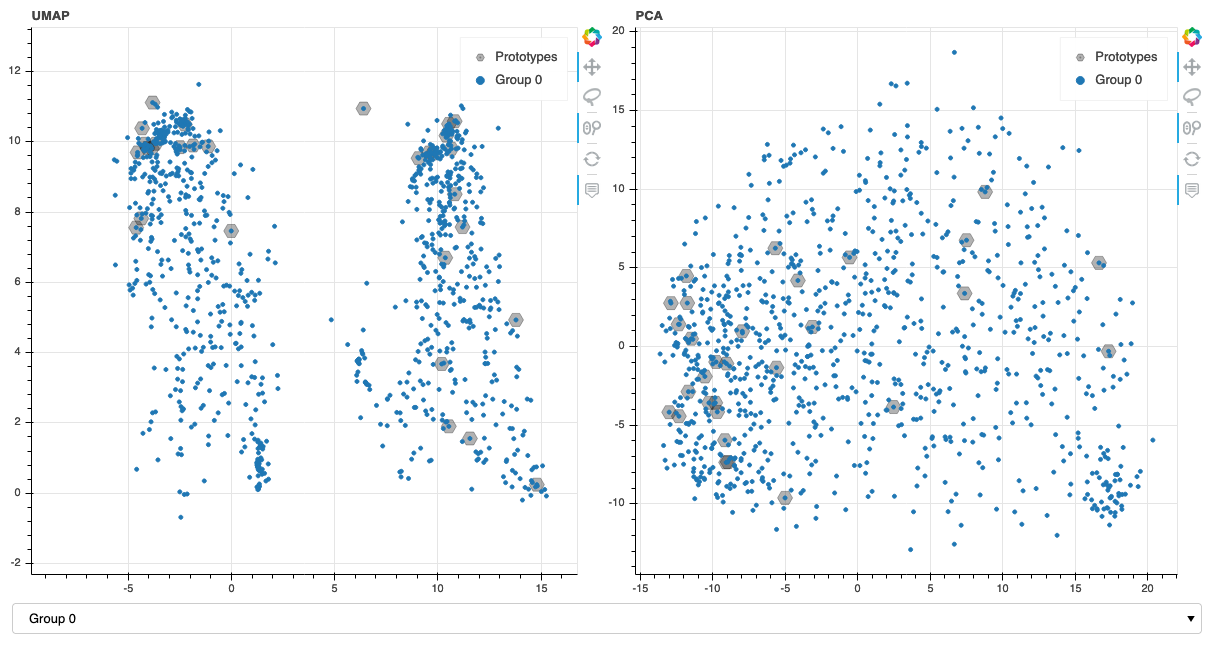
\includegraphics[width=\textwidth]{img/prototypes.png}
    \caption{Visualization of the subsample of Power Consumption dataset using PCA and UMAP. Grey hexagons highlight prototypes.}
    \label{fig:prototypes}
\end{figure}
\begin{figure}[h]
    \centering
    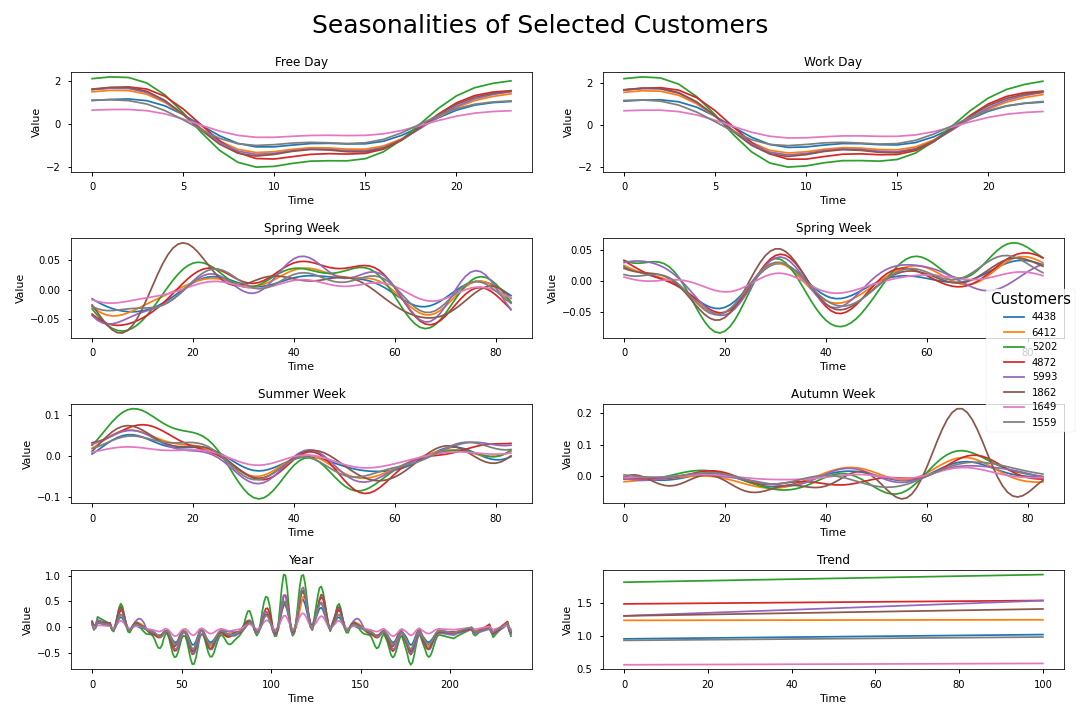
\includegraphics[width=\textwidth]{img/selected-seasonalities.png}
    \caption{Example of inspection of seasonalities and trends of selected customers using the interactive selection.}
    \label{fig:selected-seasonalities}
\end{figure}

To help with the inspection, we are providing multiple coloring options. Firstly, it is possible to select, group, and color time series manually. As this coloring is persistent throughout iterations, we can use it to study the change of positions of our time series in terms of their surroundings. Another option is to use coloring by automatic clustering or anomaly detection score. We will discuss this in the next section.

Once we are satisfied with the selected prototypes, we repeat steps 2-4 until we do not see evidence of any significant change in our visualization. Because UMAP/densMAP are stochastic, there are always some changes, but they should not be global (mixing of manually selected groups). Afterwards, we apply the MCFDTW transformation to the whole dataset.

\section{Clustering and Anomaly Detection}
As our dataset is transformed into a feature matrix, we can practically use any clustering algorithm for spatial data. In our application, the user can choose from all methods available in \textit{Scikit-learn} or \textit{HDBSCAN}. To overcome the curse of dimensionality from MCFDTW transformation and to reduce the computational time, we are using two clustering pipelines:
\begin{enumerate}
    \item We are using \textit{PCA} to reduce the number of dimensions into 50-100 dimensions based on the explained variance ratio for \textit{distance-based} clustering methods. Even though these clustering methods are not as affected by high dimensionality as \textit{density-based} methods, they usually perform better on lower dimensions.
    \item For \textit{density-based} methods \textit{OPTICS} and \textit{HDBSCAN}, we use PCA transformation into 50 dimensions followed by UMAP/densMAP embedding into 30 dimensions. As these embeddings preserve the local structure in the data, they help to overcome the sparsity of high-dimensional space.
\end{enumerate}

After the clustering, we can visualize the results in the original visualization of our dataset or its subsample (Fig.~\ref{fig:coloring-cluster}). We can use this view in prototype selection, for example, using prototypes closest to the K-means centers or discovering dense regions using HDBSCAN.
\begin{figure}[h]
    \centering
    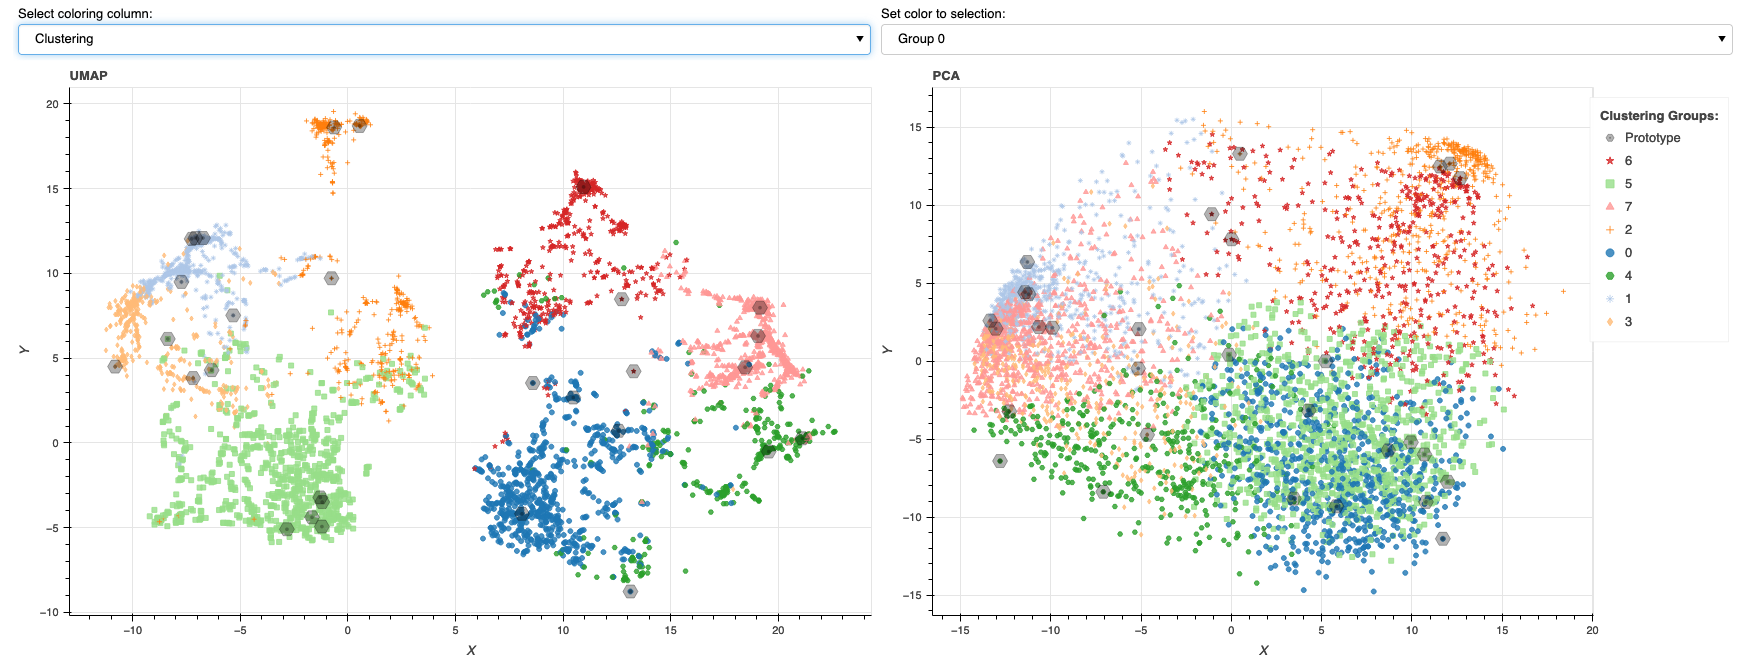
\includegraphics[width=\textwidth]{img/clustering.png}
    \caption{Using clustering from the K-means method as coloring in the visualization of a subsample of our dataset.}
    \label{fig:coloring-cluster}
\end{figure}

For detecting the anomalies in our dataset, we are using \textit{Isolation Forest} and \textit{LODA}. It is possible to use them on a whole dataset or a selected subsample. As both these methods are very efficient, we use them directly on the MCFDTW feature vector without any dimensionality reduction. Another option for anomaly detection comes from clustering with OPTICS or HDBSCAN, as both methods select certain points as noise.

Similarly to the clustering, we can plot the results of anomaly detection in our visualizations to either study their location within the dataset or to use them for identifying new potential prototypes (Fig.~\ref{fig:anomaly-detection}).
\begin{figure}[h]
    \centering
    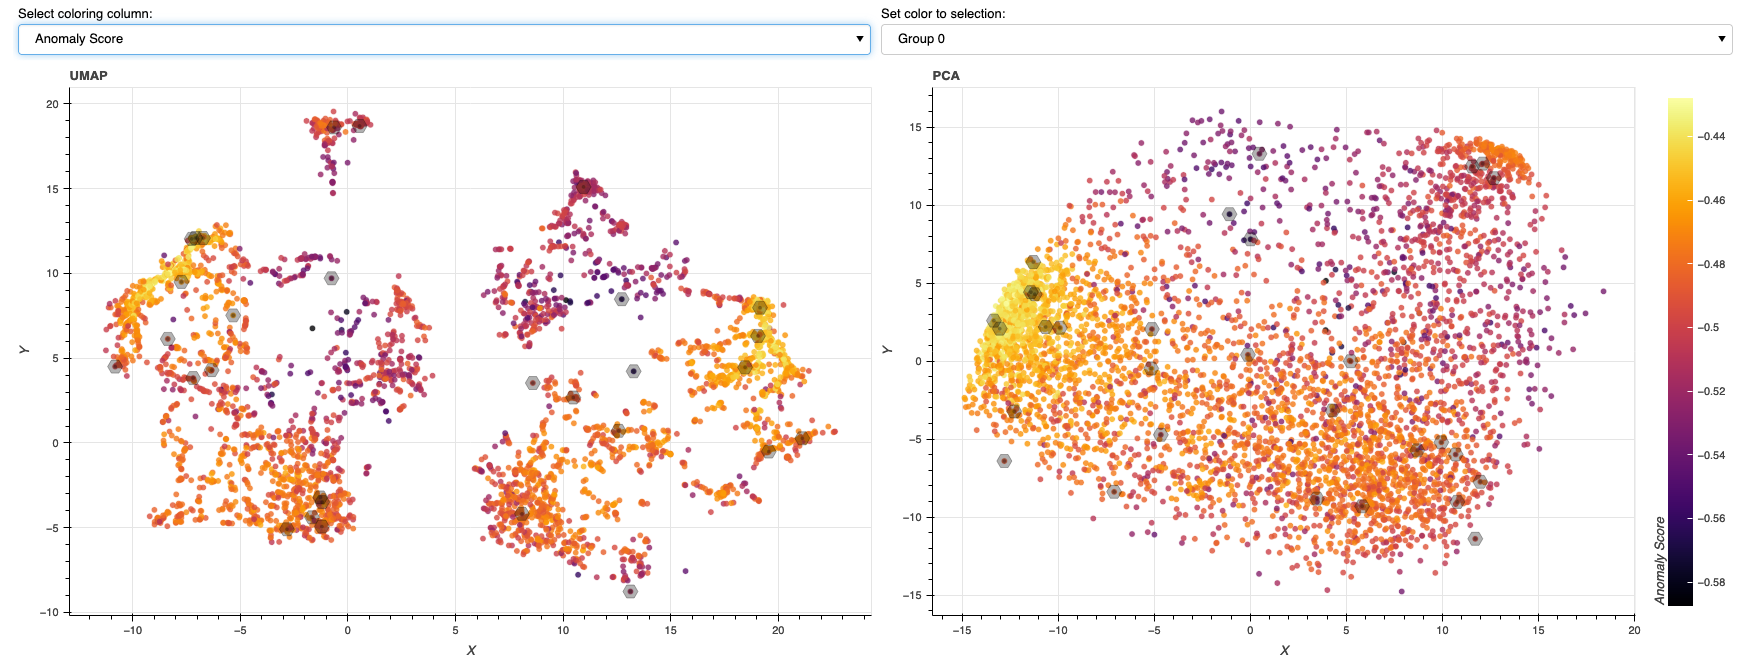
\includegraphics[width=\textwidth]{img/anomaly_detection.png}
    \caption{Coloring the data points by their anomaly score from the Isolation Forest method. The lower the value, the more anomalous is the data point.}
    \label{fig:anomaly-detection}
\end{figure}

\section{Implementation}
Our solution is mainly usable by data scientists, so we tried to use the tools that are typical and common in this field. We are using the Python programming language, and our solution is distributed as a single open-source package.

We implemented the Feature DTW and related algorithms using the well-known API defined by the \textit{Scikit-learn} project \cite{exp:sklearn_api,exp:scikit-learn}, which is the most used tool for machine learning in Python. As \textit{Scikit-learn} does not natively support work with time series, we stick to the time series interface defined by the \textit{Tslearn} library \cite{exp:tslearn}. We are using \textit{dtaidistance} \cite{exp:dtaid}, \textit{fastdtw} \cite{exp:fast-dtw-pack}, \textit{dtw-python} \cite{exp:dtw-1}, and \textit{Tslearn} \cite{exp:tslearn} python packages for computing the DTW distance and its various approximations.

Based on our knowledge of data science work, the most significant part is in the \textit{IPython} \cite{exp:ipython} and \textit{Jupyter notebooks} \cite{exp:jupyter}, and so our implementation is fully integrated into these technologies. For the visualization and rendering, we use the combination of \textit{Matplotlib} package \cite{exp:matplotlib} for smaller non-interactive visualizations, \textit{Bokeh} server \cite{exp:bokeh} for interactive visualizations, and \textit{Datashader} \cite{vis:datashader} for processing and rendering the large time series.

Even though there are some implementations of the LODA anomaly detection method, none of them is complete, and all of them lack the feature to explain the cause of the anomaly. We prepared an open-source \textit{anlearn} anomaly detection python package \footnote{\url{https://github.com/gaussalgo/anlearn}} with our implementation of LODA, that is, to the best of our knowledge, the only one containing sparse projections and the ability to explain cause of the anomaly.

As we want our work to be fully replicable, we are using the \textit{Nix} package manager \cite{exp:dolstra2008nixos} in combination with pinned requirements for all Python packages and their dependencies. This allows us to have a fully replicable work environment with the exact version of Python and all the used packages.

We were using only open-source packages in our work, and all of our source codes, including all notebooks from experiments, are available in our Github repository \footnote{\url{https://github.com/H00N24/visual-analysis-of-big-time-series-datasets}}.

\section{Results}
In our analysis, we prepared a complete processing pipeline for the large dataset of power consumption curves, starting from feature extraction and ending with data visualization, clustering, and anomaly detection.

When manually comparing time series close together in the UMAP visualization, we can see similarities in seasonalities, trends, and statistical properties. Because of this fact, we can assume that the Multi-Component Feature DTW transformation maintained properties necessary for further analysis of multi-component time series.

Upon a visual exploration, we can see two obvious larger well-separated clusters in our data (Fig.~\ref{fig:all-data-umap}). In K-means clustering, we can see that both visual clusters are divided into convex similar-sized clusters (Fig.~\ref{fig:all_data_kmeans}). In HDBSCAN clustering, we can see six clusters and a relatively large portion of noise data points (Fig.~\ref{fig:all-data-hdbscan}). Interestingly, the two large clusters from the visualization are divided very unequally. The first consists only of a single cluster, while the second one of multiple smaller clusters with noise between them.
\begin{figure}[H]
 \centering
 \begin{subfigure}[b]{0.495\textwidth}
    \centering
    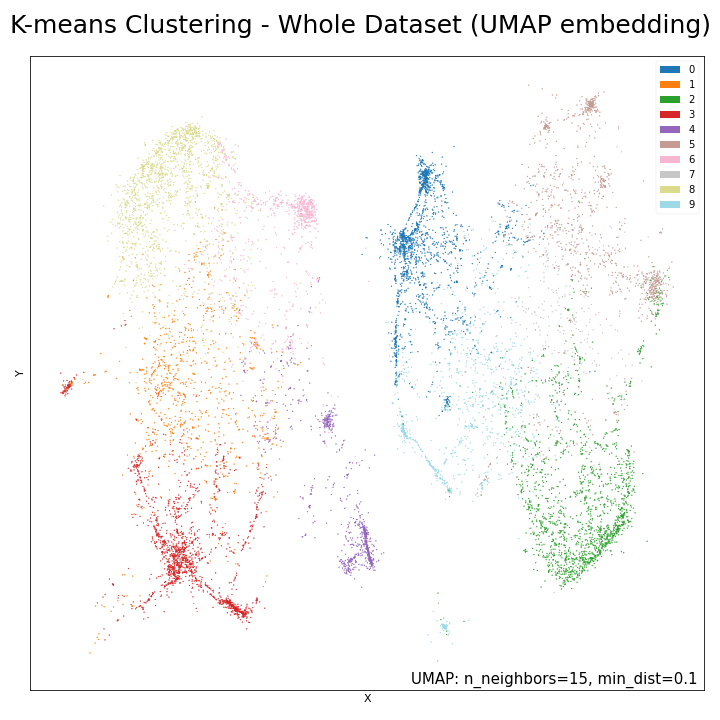
\includegraphics[width=\textwidth]{img/all-data-umap-kmeans.png}
    \caption{}
    \label{fig:all_data_kmeans}
 \end{subfigure}
 \hfill
 \begin{subfigure}[b]{0.495\textwidth}
    \centering
    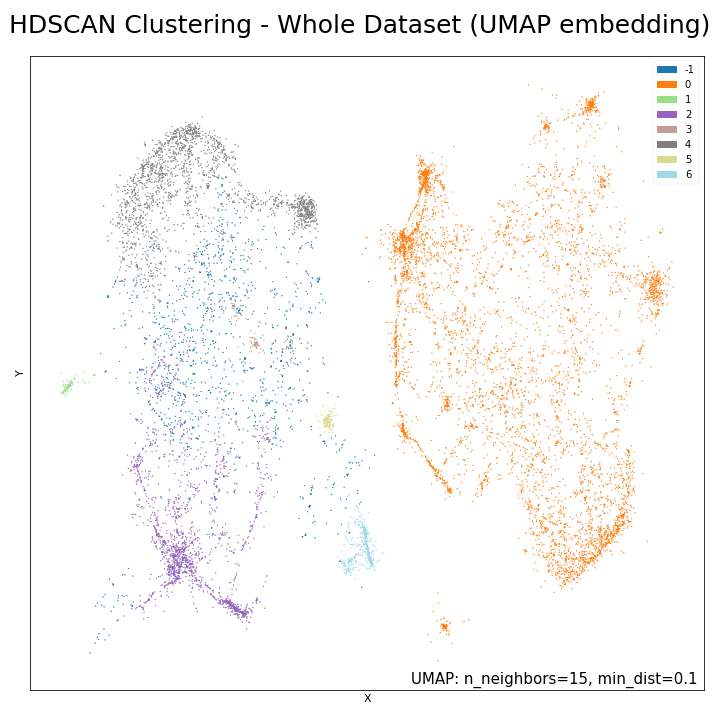
\includegraphics[width=\textwidth]{img/all-data-umap-hdbscan.png}
    \caption{}
    \label{fig:all-data-hdbscan}
 \end{subfigure}
\caption{
    (a) displays the K-means clustering on power consumption dataset. (b) shows the HDBSCAN clustering. Cluster labels are positive numbers, in HDBSCAN clustering $-1$ corresponds to noise.
}
\label{fig:all-data-umap}
\end{figure}

In anomaly detection, we used Isolation Forest and LODA methods. The results are slightly different, but we can see overlap in the group of most anomalous points. As the anomalous points have visually different power consumption curves, seasonalities, trends, and statistical properties than the rest of the points, we can consider these users to have an anomalous behavior (Fig. \ref{fig:anomalous-users}).
\begin{figure}[htp!]
    \centering
    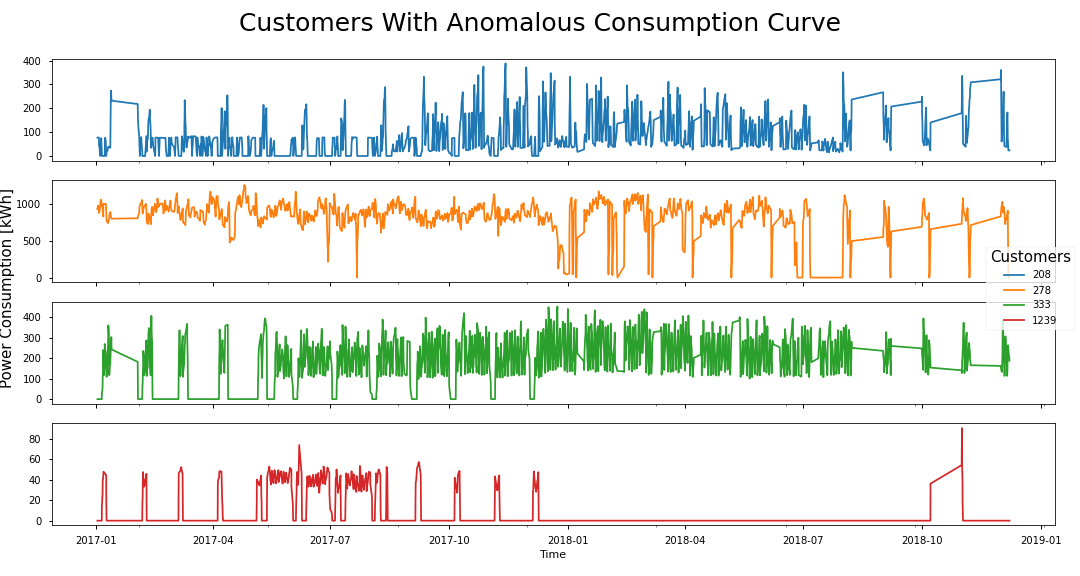
\includegraphics[width=\textwidth]{img/anomalous-users.png}
    \caption{Example of anomalous consumers detected by Isolation Forest and LODA methods. Color denotes a single customer.}
    \label{fig:anomalous-users}
\end{figure}
